\documentclass{article}

% Language setting
% Replace `english' with e.g. `spanish' to change the document language
\usepackage[english]{babel}
\usepackage{float}

% Set page size and margins
% Replace `letterpaper' with `a4paper' for UK/EU standard size
\usepackage[letterpaper,top=2cm,bottom=2cm,left=3cm,right=3cm,marginparwidth=1.75cm]{geometry}

% Useful packages
\usepackage{amsmath}
\usepackage{graphicx}
\usepackage[colorlinks=true, allcolors=blue]{hyperref}

\title{CS 520: Assignment 1 \\
\large Fast Trajectory Replanning}

\author{Swapnil Shrikrishna Verlekar (sv725)\\ Sanket Dattakumar Dalvi (sd1482)\\ Saurabh Sunil Kamble (sk2675)}

\begin{document}
\maketitle

\section*{Part 0}

We have created a maze generator class that assigns either “.” or “$\#$”. Where “.” is an unblocked cell, and “$\#$” is the blocked cell, the probability of a cell being blocked is 20$\%$ and it being open is 80 $\%$. We have fixed the start position to be the top left corner of the maze and the goal position to be the bottom right corner of the maze. For test purposes, we are running our algorithms over 50 different grid worlds randomly generated by this maze generator class.

\begin{figure}[!ht]
    \centering
    \fbox{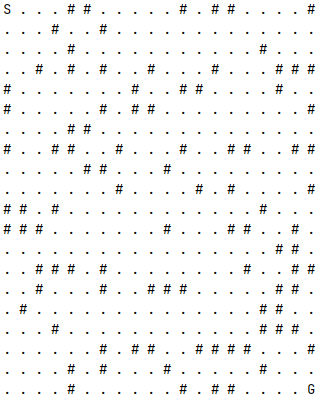
\includegraphics{part0.png}}
    \caption{Sample gird world for A* algorithm}
    \label{fig:my_label}
\end{figure}

\section*{Part 1}

\subsection*{a)}  
In the given question, the agent starts with an assumption that there are no blockers in the maze, and based on that; the agent tries to find the shortest path to the goal. Since the agent finds the goal to be three blocks away to the east, it keeps moving towards the east, observing its neighbors till it encounters a wall in its path. The agent then runs the algorithm again, considering the obstacles observed on the way to the current cell. 
For our implementation, the neighbors to the east, west, and north are explored when the agent starts exploring from the starting position. It then puts the neighbors in the open list and calculates the $f(n)$ for each of the neighbors, which is $g(n) + h(n)$. The heuristic value is calculated based on the Manhattan distance from the current position to the goal position. 
Agent then traverses to the neighbor with the least $f(n)$, which is calculated to be the East neighbor.
So, in this case, according to the given diagram, the costs for all directions are as below.

For West: 
$f(n) = g(n) + h(n);
f(n) = 1 + 4;$
$f(n)$ from the West block is 5.

For North:
$f(n) = g(n) + h(n);
f(n) = 1 + 4;$
$f(n)$ from the South block is 5.

For East:
$f(n) = g(n) + h(n);
f(n) = 1 + 2;$
$f(n)$ from the East block is 3.

So, as $f(n)$ for the east block is the lowest among all, the first move of agent will be east rather than in other directions.

\subsection*{b)}
For our algorithm, we add the agents current position to our closed list (contains all the nodes we have expanded) so that it will not be visited again. Then we begin by exploring neighbors from the agent's current position. We check whether all the neighbors are inside the wall (within the bound) and are not blockers. If it is not a blocker and not present in the closed list then we add them to our open list (priority queue implemented using heap). Otherwise, if neighbor is already present in the open list we will update its corresponding values $f(n), g(n), h(n);$ if the new $f(n)$ is lesser than the previous $f(n)$, then same process is repeated for the its neighbors.
For example in a 100 x 100 maze the agent will expand:
$1 \le Nodes Expanded \le 10000$.
Hence, in the finite grid world our agent will take finite time to either reach the goal or discover that it is impossible to to reach the target. In worst case scenario our agent will traverse the entire maze. So for an $n*n$ maze, the maximum number of nodes it can explore is $n^2$.

\section*{Part 2}

In our Repeated Forward A* algorithm, when we resolve the ties between f-values using the g-values, it is observed that the selection of a node with a large g-value leads to the algorithm running comparatively faster when it comes to the execution time and also lesser number of nodes are expanded. 
For our algorithm we are selecting the node with minimum $f(n)$ value from the open list (priority queue) to explore and when the larger g-value is selected, then the heuristic value will in-turn smaller $(f(n) = g(n) + h(n))$. Choosing a larger g-value means we are choosing the node that is already closer to the goal since we always travel in the direction towards the goal unless the path in the direction to it is blocked, in which case we go around the blocked cell. Inversely, choosing a smaller g-value would take a longer time to reach the goal, since the g(n) is smaller its further away from the goal. Therefore breaking ties in $f(n)$ with larger g-values leads to finding a path to the goal faster since we will be expanding less number of nodes.

\begin{figure}[!ht]
    \centering
    \fbox{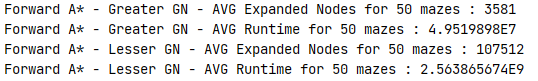
\includegraphics[width=\linewidth]{part2.png}}
    \caption{A* run-time with larger g(n) value against smaller g(n) value}
    \label{fig:my_label}
\end{figure}

For 50 101*101 grids, implementing heap that breaks f-value ties in favor of larger g-values expanded on an average 3581 nodes but the heap in favor of smaller g-values expanded on an average 107512 nodes which is more by a factor of 30.
And the run-time is more by a factor of about 60.


\section*{Part 3}

After implementing and comparing both the algorithms we observed that Repeated Forward A* is faster compared to our Repeated Backward A* since the number of nodes expanded by the Backward A* is much larger than the number of nodes expanded by Forward A*. This is because the agent is closer to the Start, the Repeated Backward A* has less information, which necessitates fewer restarts for the Repeated Forward A* while the Backward A* does not become aware of the wall/blockers until it comes near to the beginning.

For 50 mazes of 101x101, we can observe that the Forward A* Expands 5 times lesser nodes and runs 11 times after than Backward A*  

\begin{figure}[!ht]
    \centering
    \fbox{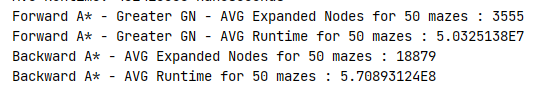
\includegraphics[width=\linewidth]{part3.png}}
    \caption{Run-time for Forward A* and Backward A*}
    \label{fig:my_label}
\end{figure}

\section*{Part 4}

Manhattan distance between any two cells in the grid is given by ${|(x1 - x2)}| + |{(y1 - y2)|}$ which is vertical or horizontal path. And similarly our agent can only move in 4 compass directions north (vertically up), south (vertically down), east (horizontally right), west (horizontally left) therefore Manhattan gives the shortest path for our agent to reach the goal. Hence, the Manhattan distance is consistent.

A heuristic function is called consistent, if the following holds true: $\forall (n,a,n'): h (n)\leq c(n,a,n')+h(n')$, where $\ c(n,a,n')$ is step cost for going from $\ n$ to $\ n'$ using action $\ a$. In order to prove that “the Manhattan distances are consistent in grid-worlds in which the agent can move only in the four main compass directions.”, we will consider two cases. The first case is, if the cell $\ n$ is closer to the target cell than the cell $\ n'$. In this case, the $\ h(n) \leq h(n') \implies h(n) \leq h(n')+c(n,a,n')$ since it is located closer to the target cell. The second case is if the cell $\ n'$ is located somewhere between the cell $\ n$ and the target cell. In this case, $\ h(n') \leq h(n)$, since it is closer to target cell. However, since $\ c(n,a,n')$ is the cost for going from $\ n$ to $\ n' \implies h(n) \leq h(n')+c(n,a,n')$ because after getting from $\ n$ to $\ n'$, the rest of the path to the target cell cannot be more than $\ h(n')$.

And because every time the Adaptive A* algorithm is ran and $\ h_{new}(s)$ is calculated, it updates the $\ h(s)$ not only of the cell where the agent is located, but for all of the cells that it expanded on its way to the target cell from the agent's cell. Therefore, the h-values $\ h_{new}(s)$ are not only admissible but also consistent.\cite{1}

\section*{Part 5}

When we run both the algorithms Repeated Forward A* and Adaptive A* on 50 grids of 101 X 101 size, we can observe that the run-time of Adaptive A* is less, i.e., Adaptive A* finds the path faster when it is compared to Repeated Forward A*.

The reason behind it is that for Adaptive A*, the algorithm uses a modified heuristic which is calculated as a difference between the goal’s g(n) and the current node’s g(n). This leads to a more realistic heuristic value that is admissible and closer to the actual heuristic. 

\begin{figure}[!ht]
    \centering
    \fbox{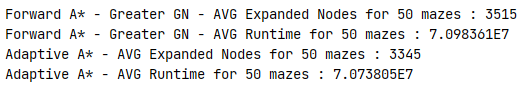
\includegraphics[width=\linewidth]{part5.png}}
    \caption{Run-time for Forward A* and Adaptive A*}
    \label{fig:my_label}
\end{figure}

The Adaptive A* algorithm does not expand as many cells as the Repeated Forward A* because each time it finds the path to the target cell, it updates the h(n) of cells in the closed list. Therefore, when the agent follows that path, runs into a blocked cell, and reruns the algorithm to find a new path, then the algorithm would use the updated h(n) from the previous iteration of A* and this new search will be more focused and informed.\cite{4}

In the above run, we can observe that Adaptive A* expands 5$\%$ lesser nodes than Forward A*
   

\section*{Part 6}

For our Statistical hypothesis test, we are going to use the Repeated Forward A* for the algorithm with larger g-values as tie-breakers and the Repeated Forward A* algorithm with smaller g-values.

We can perform the Null Hypothesis test to determine if the A* algorithm with larger g-values runs faster than the A* algorithm with smaller g-values. Therefore, our Null Hypothesis is that the difference in the run-time is only due to sampling noise otherwise both algorithms have the same run-time.\cite{2}

Thus we will calculate the p-value and if the p-value is less than 0.05 then we typically consider it to be statistically significant, in which case the null hypothesis is rejected.

We will use this hypothesis to decide whether the algorithm is systematic in nature. We can run both the algorithm on a very large population of girds of size 101 x 101 and based on the results we will either reject the Null Hypothesis (i.e the difference is not due to sampling noise and algorithms are systematic in nature) or we will fail to reject the Null Hypothesis. For our implementation of running the two algorithms, the repeated forward A* algorithm with larger g-values was much faster than the one with smaller g-values over a very large population hence we can confidently reject the Null Hypothesis and say that the result is due to the Systematic nature of the two algorithms.\cite{3}

\bibliographystyle{alpha}
\bibliography{sample}

\end{document}